\subsection{Optimizations for PPA}\label{sec:computingprobabilitiesOptimizations}

While model counting and solution space quantification are general problems, their application to probabilistic program analysis can often be improved exploiting the additional information specific to this application field.

Without any sake of completeness, we will briefly report in this section two techniques able to 1) exploit variables dependency to reduce the complexity of model counting and solution space quantification and 2) combine interval constraint propagation and stratified sampling to increase the accuracy of sampling-based probability computation, and in turn its convergence rate.

\mycomment{Anto: the next may need some serious reworking}

\paragraph{Divide and conquer.}
The complexity of all the model counting and solution space quantification techniques proposed in this section depends on the number of variables involved in the constraints to be quantified. Let us assume such constraints are provided in disjunctive normal form and that there is no intersection between the solution spaces of any pair of disjuncts (this is form is quite natural for most constraints analyzed in PPA, usually requiring low computational overhead for normalization). Since there is no intersection between the disjuncts, the solution space for each of them can be quantified separately and than summed up to obtain the result for the whole disjunction.

Let us focus on a single disjunct $\phi \equiv \phi_1 \land \phi_2 \land \dots \land \phi_n$ predicating on the variables $\{v_1, v_2, \dots, v_m\}$, i.e., for each $v_i$ there exists at least one conjunct $\phi_j$ predicating on its value. Our goal is to divide the quantification of the solution space of $\phi$ in a set of independent problems involving only a subset of the variables appearing in $\phi$. 

The central idea is that constraints in $\phi$ identify a dependency relation ($\textit{dep}$) among the constrained variables that can be formalized as follows (let $v_i$, $v_j$, and $v_k$ be variables in $\phi$ and $\phi_i$ be a conjunct in $\phi$):
\begin{itemize}
	\item $\forall v_i \ \textit{dep}(v_i,v_i)$
	\item $\forall v_i,v_j$ if there exist a conjunct $\phi_i$ predicating on both $v_i$ and $v_j$, then $\textit{dep}(v_i,v_j)$
	\item $\forall v_i,v_j,v_k$ $\textit{dep}(v_i,v_j) \land \textit{dep}(v_j,v_k) \implies \textit{dep}(v_i,v_k)$
\end{itemize}

The intuitive meaning of the $\textit{dep}$ relation is that if $\textit{dep}(v_i,v_j)$ then the values assumed by $v_i$ in a program run affect the values that can be assumed by $v_j$ towards the satisfaction of $\phi$. For example, from $\{x>5 \land y=x+5\}$ we deduce that the value of $y$ is affected by the values of $x$, and vice versa. The relation $\textit{dep}$ is an equivalence relation, thus it induces a partition on the set of variables appearing in $\phi$. For this reason, we can rewrite $\phi$ as the conjunction of the subsets $\phi_{[v]}$, each of whom collects all the constraints involving a variable in the equivalence class of $\textit{dep}$ represented by $v$. Such conjuncts are logically separated, hence it can be proved that $\textit{Pr}(\phi)= \prod_{v} \textit{Pr}(\phi_{[v]})$. 

For example, let $\phi$ be $\{x>2 \land y<5\}$, its probability can be computed as $\textit{Pr}(\phi)=\textit{Pr}(x>2) \cdot \textit{Pr}(y<5)$. The computation of the two probabilities on the right-hand side of this equality can be performed independently and each of them involves only one variable, reducing the effort of counting in a multidimensional space or taking samples from multidimensional distributions. Furthermore, the result of each subproblem can be cached and reused, with significant benefits in practical applications~\cite{Filieri2013}.


%\paragraph{Sampling effort allocation.}
%\mycomment{Anto: this is probably too advanced. Maybe enough to refer the students to the fse15 paper}

\paragraph{Interval constraint propagation and stratified sampling.}

Recall the example we introduced in Section~\ref{sec:computingprobabilitiesSampling}: we aim at quantifying the probability of satisfying the constraint 
$v_1 \leq -v_2 \land v_2 \leq v_1$, where both $v_1, v_2 \in [-1, 1] \cap \mathbb{R}$. Figure~\ref{fig:stratifiedICP} shows the domain and the solution space for this problem, with $v_1$ on the x-axis and $v_2$ on the y-axis. Using hit-or-miss Monte Carlo to solve this problem requires throwing random samples for $v_1$ and $v_2$ within their domain (i.e., from within the square), and computing the ratio between those falling within the shadowed triangle (i.e., satisfying the constraints) and the total number of samples. Geometrically, this corresponds to estimating the ratio between the area of the triangle and the area of the square (which is 1/4).

\begin{figure}[h!]\label{fig:stratifiedICP}
  \centering
      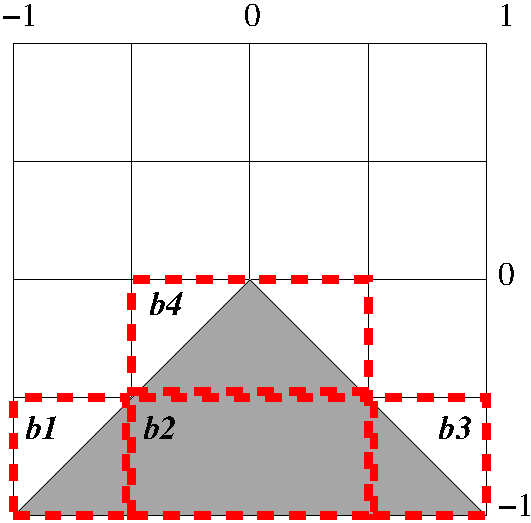
\includegraphics[width=3cm]{triangle}
  \caption{ICP-based stratified sampling.}
\end{figure}

However, looking at the figure it is clear already before sampling that some regions of the domain do not contain solutions, thus every input value sampled from those regions will not satisfy the constraint. In other words, the probability of satisfying the constraint within those regions is identically 0, without any estimation uncertainty. 
